% !TeX root = RJwrapper.tex
\title{An Open-Source Implementation of the CMPS Algorithm for Assessing
Similarity of Bullets}
\author{by Wangqian W. Ju and Heike Hofmann}

\maketitle

\abstract{%
In this paper, we introduce the R package \pkg{cmpsR}, an open-source
implementation of the Congruent Matching Profile Segments (CMPS) method
developed at the National Institute of Standards and Technology (NIST)
for objective comparison of striated tool marks. The functionality of
the package is showcased by examples of bullet signatures that come with
the package. Graphing tools are implemented in the package as well for
users to assess and understand the CMPS results. Initial tests were
performed on bullet signatures generated from two sets of 3D scans in
the Hamby study under the framework suggested by the R package
\pkg{bulletxtrctr}. New metrics based on CMPS scores are introduced and
compared with existing metrics. A measure called Sum of squares ratio is
included, and how it can be used for evaluating different scans,
metrics, or parameters is showcased with the Hamby study data sets. An
open-source implementation of the CMPS algorithm makes the algorithm
more accessible, generates reproducible results, and facilitates further
studies of the algorithm such as methods comparison.
}

\newcommand{\hh}[1]{{\textcolor{orange}{#1}}}
\newcommand{\wj}[1]{{\textcolor{blue}{#1}}}
\setlength{\parindent}{0pt}

\hypertarget{introduction}{%
\subsection{Introduction}\label{introduction}}

In this paper we present an open-source implementation of the algorithm
of the Congruent Matching Profile Segments (CMPS) method. \citet{cmps}
developed the CMPS method for ``objective comparison of striated tool
marks'' and demonstrated its use in some examples of comparing bullet
signature correlations. Although \citet{cmps} conceptually described the
CMPS algorithm in their paper, the authors did not release an
implementation of their method. Thus, our effort here is to introduce
the CMPS method to the \texttt{R} \citep{R} community and provide an
open-source, publicly available implementation of the algorithm to use,
review, and improve. Our implementation is made available as part of the
\texttt{R} package \pkg{cmpsR} on GitHub at
\url{https://github.com/willju-wangqian/cmpsR}.

According to the Uniform Crime Reporting Program of FBI (Federal Bureau
of Investigation), ``More than 73 percent (73.7) of the homicides for
which the FBI received weapons data in 2019 involved the use of
firearms'' \citep{fbiucr}, and firearm examination could play an
important role in all these cases. \textbackslash hh\{XXX the new data
for 2020 came out on Sep 27 - homicides are up by close to 30\%. We
might want to mention that.\} An important task of firearm examination
is to answer the question of whether two pieces of evidence come from
the same source or whether a piece of evidence matches a sample obtained
from a specific firearm. Here, in particular, we are interested to
determine whether two bullets were fired from the same gun barrel.
Assessing the similarity between two bullets is based on a comparison of
striation marks acquired during the firing process as bullets are
propelled through the barrel. Current state of art sees firearms
examiners make an assessment of similarity based on a visual comparison,
generally, using a comparison microscope \citep{afte}. This practice has
been criticized for its lack of objectivity and the associated problem
in calculating an error rate \citep{pcast}.

A report published by \citet{nrc} states that ``{[}m{]}uch forensic
evidence-including, for example, bite marks and firearm and toolmark
identification---is introduced in criminal trials without any meaningful
scientific validation, determination of error rates, or reliability
testing to explain the limits of the discipline.'' To overcome those
criticisms and concerns, researchers have been making an effort to build
databases and develop frameworks and algorithms that bring an objective
and quantitative assessment into the field
\citetext{\citealp[\citet{brundage}, \citet{hamby}, \citet{Hamby:2019},
\citet{song2005}, \citet{ChumbleyL_Scott2010VoTM}, \citet{aoas},
\citet{pmid30444940}]{nistdb}; \citealp{cmps}}. Note that this is not an
exhaustive list of these efforts. The notion of bullet signatures is one
of the results of these efforts. Bullet signatures can be extracted from
bullet land engraved areas (LEAs), typically one for each land engraved
area, and how those bullet signatures are extracted from scans will be
discussed in the Background section. Since bullet signatures can
numerically describe the striation marks on the bullet and can be
understood by algorithms, they played an important role in bringing
objectivity into the field. In the following sections we will: review
the background of bullet signature comparisons, discuss how we followed
the idea described by \citet{cmps} for the implementation of the CMPS
algorithm, propose new metrics based on the CMPS score and a principled
evaluation framework for algorithmic results comparison, and present
results of applying our implementation to real data.

\hypertarget{background}{%
\subsection{Background}\label{background}}

\textbf{Hamby data set}

The datasets we worked with come from the James Hamby Consecutively
Rifled Ruger Barrel Study \citep{brundage, hamby, Hamby:2019}, in
particular, Hamby set 252 and Hamby set 44. For each Hamby set, a total
of 35 bullets is fired from (the same) ten consecutively manufactured
Ruger P-85 pistol barrels. Two bullets are fired from each barrel,
making up a set of 20 reference bullets. An additional 15 bullets are
fired from these ten barrels in a fashion unknown to the study
participant. The aim of the Hamby Study was to have firearms examiners
identify which barrel each of the 15 questioned bullets was fired from.
The Ruger P-85 barrels are traditionally rifled barrels with six grooves
and lands as shown in \autoref{fig:bullet}. During the firing process,
grooves and lands are engraved on a bullet. Firearms examiners use
striation marks on land engraved areas (LEAs) for their visual
comparison. For algorithmic purposes, 3D topographical images of land
engraved areas were obtained and stored in x3p format (XML 3-D Surface
Profile). The x3p format provides a standard way of exchanging 2D and 3D
profile data. It conforms to the ISO5436-2 standard
{[}\url{http://sourceforge.net/p/open-gps/mwiki/X3p/}{]} adopted by the
OpenFMC (Open Forensic Metrology Consortium), a group of firearm
forensics researchers who contributes to the establishment of best
practices of using metrology in forensic science. Hamby set 252 were
scanned using a NanoFocus lens at 20x magnification with the scan
resolution being 1.5625 \textmu m \(\times\) 1.5625 \textmu m per pixel.
Hamby set 44 was scanned at the Roy J Carver High-Resolution microscopy
lab at Iowa State. These scans were acquired with a Sensofar Confocal
Light Microscope at 20x magnification for a nominal resolution of 0.645
\textmu m \(\times\) 0.645 \textmu m per pixel. Both Hamby set 252 and
Hamby set 44 are publicly available on the NIST Ballistics Database
Project \citep{nistdb}.

\textbf{Extracting signatures from LEA scans}

The automated framework used in this paper was proposed by \citet{aoas}.
In order to obtain bullet signatures from the x3p files of bullet land
engravings, we use the \texttt{R} packages \pkg{x3ptools}
\citep{x3ptools} and \pkg{bulletxtrctr} \citep{bulletxtrctr}.
\pkg{x3ptools} is a package to read, write, and generally, process x3p
files. The \pkg{bulletxtrctr} package implements a pipeline for
extracting and comparing signatures from scans of land-engraved areas.

\autoref{fig:process} gives an overview of all of the steps in the
process from scan to signatures. \autoref{fig:process}(a) shows a
rendering of a 3d scan of a bullet land engraved area. The raised
portion of the surface on the left and right of the scan are parts of
the adjacent groove engraved areas (GEAs), the middle area shows a
land-engraved area (LEA) with well expressed striation marks. The first
step of obtaining the bullet signature is to extract a cross-section at
a fixed height along the land engraving.

The white horizontal line in \autoref{fig:process}(a) indicates which
cross-section was identified by the algorithm to represent the LEA;
\autoref{fig:process}(b) shows the corresponding cross-sectional view.
Groove engraved areas are removed from the analysis as indicated by the
vertical blue lines in \autoref{fig:process}(c) and
\autoref{fig:process}(d)). A non-parametric LOESS smooth \citep{loess}
is fitted to capture the bullet curvature (\autoref{fig:process}(e))
and, finally, the \textbf{bullet signature} (\autoref{fig:process}(f))
is obtained as residuals of the cross-section and the fitted smooth.
Note, that in \citet{cmps} bullet signatures are referred to as bullet
profiles. However, to avoid confusion, we distinguish the notion of
bullet signatures from bullet profiles. Bullet profiles are shown in
panels (b), (c), and (d) of \autoref{fig:process}, while
\autoref{fig:process}(f) shows the corresponding bullet signature.
Identifying the groove engraved areas correctly is fundamental for a
correct down-stream analysis of the signatures. To allow for a
human-in-the middle inspection and intervention we have provided an
interactive web-application, implemented as \texttt{R} Shiny App
\citep{shiny}, \pkg{bulletinspectR} to identify and correct those
errors. An example of the extraction process with corresponding code and
parameter settings can be found on Github at
\url{https://github.com/willju-wangqian/CMPSpaper/tree/main/reproducible}.
Note that the process of extracting signatures might be different from
the one used in \citet{cmps} because no code or parameter settings are
made available publicly.

\begin{Schunk}
\begin{figure}

{\centering 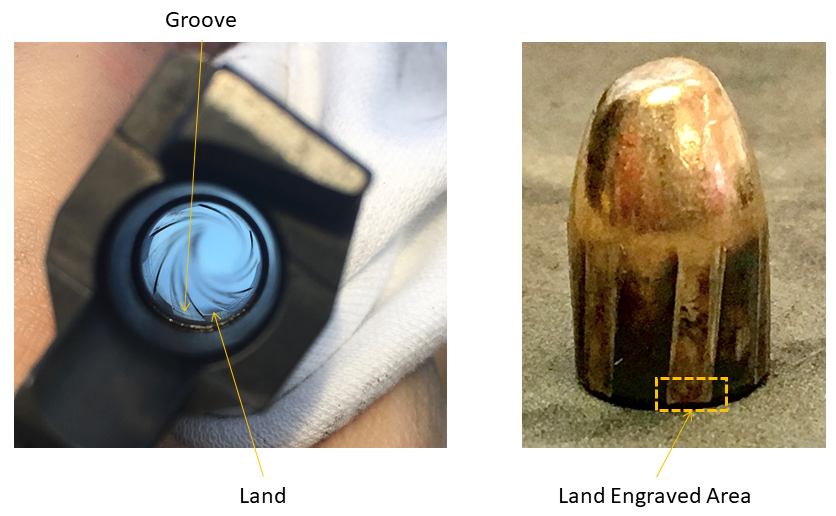
\includegraphics[width=.8\textwidth]{ju-hofmann_files/figure-latex/barrel_bullet_ps} 

}

\caption[Photo of a traditionally rifled gun barrel (left) and a fired bullet (right)]{Photo of a traditionally rifled gun barrel (left) and a fired bullet (right).}\label{fig:bullet}
\end{figure}
\end{Schunk}

\begin{Schunk}
\begin{figure}

{\centering 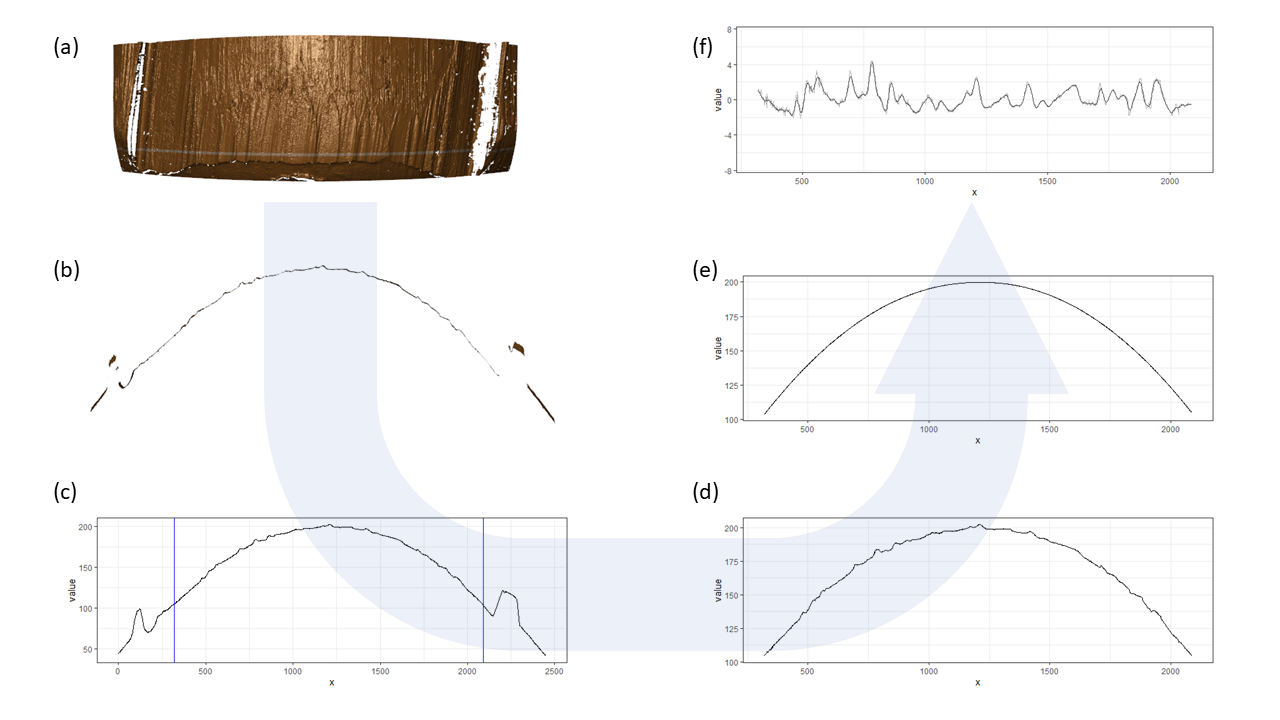
\includegraphics[width=.9\textwidth]{ju-hofmann_files/figure-latex/figure1_v2} 

}

\caption[A framework of obtaining a bullet signature]{A framework of obtaining a bullet signature. (a) front view of a scanned land engraved area (LEA). The selected crosscut location is indicated by the white line. (b) view of the cross-section of the land engraved area at the white line in (a). (c) the crosscut data plotted in 2D; blue vertical lines indicate the position of left and right grooves. (d) the crosscut data after chopping the left and right grooves. (e) the fitted curvature using LOESS. (f) after removing the curvature from the crosscut data, the bullet signature is obtained}\label{fig:process}
\end{figure}
\end{Schunk}

\textbf{Conceptual idea of CMPS}

Most algorithms for comparing striation marks are based on the digitized
signatures and produce a similarity score
\citep[\citet{ChumbleyL_Scott2010VoTM}, \citet{aoas},
\citet{pmid30444940}]{song2005}. The congruent matching profile segments
(CMPS) algorithm, developed by \citet{cmps} for ``objective comparison
of striated tool marks'', is one such algorithm. The algorithm's main
idea is to take a set of consecutive and non-overlapping basis segments
from the comparison and for each segment find the ``best'' registration
position on the reference (the other bullet signature) with respect to
their cross-correlation values. From a comparison of these registration
positions, a \textbf{congruent registration position} is identified, and
the number of basis segments taking the congruent registration position
is the CMPS score. Note that researchers in \citet{cmps} refers to the
origin of basis segments as the reference, but in this paper we refer to
it as the comparison. High CMPS scores are achieved between more similar
signatures and are therefore indicative of a same-source pair. Low
scores between pairs of signatures are attributed to different source
pairs. However, a specific threshold of the CMPS score to distinguish
between same-source and different-source comparisons is not provided in
\citet{cmps}, instead the threshold depends on the underlying structure
of the data and the choice of parameters.
\hh{XXX  In a legal setting this variability is problematic because it allows for situations in which experts could choose parameters based on a wished-for outcome. }
Further research is needed to understand how to determine optimal
threshold settings. The CMPS algorithm can assist firearm examiners with
drawing a conclusion about the source of a comparison pair.
Unfortunately, \citet{cmps} did not release any code or specific
parameter settings for their implementation of the CMPS algorithm. Thus,
in this paper we present an open-source implementation of the CMPS
algorithm in the R package \pkg{cmpsR} available from Github
\url{https://github.com/willju-wangqian/cmpsR}. This publicly available
implementation calculates the CMPS score of a comparison using the
following code:

\begin{Schunk}
\begin{Sinput}
# install.packages("devtools") 
# devtools::install_github("willju-wangqian/CMPS")

library(cmpsR)
data(bullets)

sig1 <- bullets$sigs[[2]]$sig
sig2 <- bullets$sigs[[9]]$sig
sig3 <- bullets$sigs[[10]]$sig

cmps.result.KM <- extract_feature_cmps(sig1, sig2)
cmps.result.KNM <- extract_feature_cmps(sig1, sig3)
\end{Sinput}
\end{Schunk}

In this example, the comparison between \code{sig1} and \code{sig2}, two
signatures coming from the same source (a known-match comparison), gets
a CMPS score of 17; the comparison between \code{sig1} and \code{sig3},
two signatures coming from different sources (a known non-match
comparison), gets a CMPS score of 1.

We also implemented graphing tools for users to better understand these
results as well as the algorithm itself.

The section ``Implementation'' will go through the algorithm and show
how to use the \pkg{cmpsR} package. A further example that illustrates
the main points is also included. The section ``Results'' presents the
results of evaluating the \pkg{cmpsR} package using Hamby set 252 and
Hamby set 44. The results from Hamby set 252 are used to verify that our
implementation is, at least qualitatively, comparable to the algorithm
described in \citet{cmps}. Results from Hamby 44 show the need for a
further investigation of the parameter choices even in the case of
bullets fired from the same barrels.
\wj{We suggest new CMPS metrics that summarize land-level CMPS scores and a sum of squares ratio that can be used to evaluate algorithmic results.}
The last section covers some final discussion and conclusions.

\hypertarget{implementation}{%
\subsection{Implementation}\label{implementation}}

\textbf{Algorithm}

Conceptually, the CMPS algorithm consists of three main steps:

\begin{enumerate}
\def\labelenumi{\arabic{enumi}.}
\item
  \textbf{cut the comparison signature into consecutive, non-overlapping
  and equal-length basis segments:} The command
  \code{get\_segs(x, len=50)} implements this step: it takes bullet
  signature \code{x} in the format of a numeric vector and cuts it into
  consecutive, non-overlapping and equal-length segments of length
  \code{len}, which are referred to as ``basis segments''.
\item
  \textbf{identify candidate positions:} For each basis segment a set of
  candidate registration positions on the comparison signature is
  identified based on the segment's similarity to the reference
  signature. In a first step, the cross-correlation function of the
  segment to the reference is calculated, then a number of positions
  with high correlation values are identified as candidate positions. In
  case multiple segment lengths are considered, the length of each basis
  segment is expanded (by default it is doubled) and these two steps are
  repeated. Only when candidate positions coincide (or are similar
  enough), they are considered further. \autoref{fig:segplots} and
  \autoref{fig:seg_all} illustrate these ideas.

  \begin{itemize}
  \item
    \textbf{Calculate the cross-correlation curve:} Calculate the
    cross-correlation curve between a basis segment \code{x} and the
    reference signature \code{y} using the function
    \code{get\_ccf4(x, y, ...)} as shown in \autoref{fig:segplot2}. The
    position indicates the lag by which a basis segment is moved with
    respect to its original placement. A position is considered ``good''
    if it results in a peak in the cross-correlation between the basis
    segment and the reference.
  \item
    \textbf{Correlation peaks:} Two strategies referred to as
    ``multi-peak inspection'' and ``multi-peak inspection at different
    segment lengths'' in \citet{cmps} are used for identifying positions
    of correlation peaks as candidate positions. The latter is also
    called ``multi-segment lengths strategy''. The parameter
    \code{npeaks.set} in \code{extract\_feature\_cmps(...)} determines
    which strategy to use and the number of candidate positions:

    \begin{itemize}
    \tightlist
    \item
      If \code{npeaks.set} is an integer vector of length 1, for example
      \code{npeaks.set = 5}, the positions of the top five peaks in the
      cross-correlation curve are identified as candidate positions for
      registration.
    \item
      If \code{npeaks.set} is an integer vector of length more than 1,
      for example \code{npeaks.set = c(5, 3, 1)}, the multi-segment
      lengths strategy will be used: calculate the cross-correlation
      function between a basis segment and the reference and identify
      positions of the top five peaks; double the segment length to a
      specified value, re-calculate the cross-correlation function, and
      identify three peaks; repeat this process and identify a single
      peak in the newly computed cross-correlation function.
      \autoref{fig:seg_all} shows an example of three levels of basis
      segment 6 and their corresponding cross-correlation curves and
      identified peaks. Note that in \citet{cmps} the segment length is
      doubled at each level of a basis segment, but in the present
      implementation users are allowed to choose the segment length at
      each level.
    \item
      \code{get\_ccr\_peaks(comp, segments, seg\_outlength, nseg = 1, npeaks = 5)}
      computes the cross-correlation curve between a basis or increased
      segment and the reference signature and finds peaks in the
      cross-correlation curve. The number of peaks detected is equal to
      \code{npeaks}, which is an integer. \code{segments},
      \code{seg\_outlength}, and \code{nseg} determines the segment in
      the cross-correlation computation, and \code{comp} gives the
      reference signature. If the multi-segment lengths strategy is
      used, then \code{get\_ccr\_peaks(...)} is called in a
      \code{lapply()} for each level of the basis segment. The resulting
      list is called \code{ccr.list}.
    \end{itemize}
  \item
    \textbf{multi-segment lengths strategy:} with the multi-segment
    lengths strategy being used, a position is identified as a candidate
    position for registration and is called as a ``consistent
    correlation peak'' if it results in a top peak in the
    cross-correlation curve with a tolerance zone determined by
    \code{Tx} in all segment levels. Note that in \citet{cmps}, a
    segment at its largest scale (highest level) always identifies one
    peak, but we do not have this requirement in our implementation.

    \begin{itemize}
    \tightlist
    \item
      the function \code{get\_seg\_scale(segments, nseg, out\_length)}
      is used to obtain the (potentially increased) version of a basis
      segment. \code{segments}, which is a list containing all basis
      segments generated by the function \code{get\_segs(...)} in step
      1, and \code{nseg} are used to determine the basis segment to be
      increased. \code{out\_length} specifies the length of the output
      segment.
    \item
      \code{get\_ccp(ccr.list, Tx = 25)} tries to identify the
      ``consistent correlation peak''. \code{ccr.list} is the result of
      \code{lapply()} and \code{get\_ccr\_peaks(...)}, and \code{Tx}
      determines the size of a tolerance zone used in identifying the
      consistent correlation peak. \code{get\_ccp(...)} returns
      \code{NULL} if there is no consistent correlation peak.
    \end{itemize}
  \end{itemize}
\item
  \textbf{determine the congruent registration position:} A candidate
  position ``receives'' votes from basis segments that identify it or a
  close position within a tolerance zone of \code{Tx} as a candidate
  position in step 2. Votes for all candidate positions are tallied, and
  the position with the highest number of votes gets chosen as the
  \emph{congruent registration position}, indicating that most of the
  basis segments find their highly similar counterpart in the reference
  signature in terms of correlation at this registration position. In
  case of ties the middle position is taken as the congruent
  registration position. Basis segments with a congruent registration
  position are called ``congruent matching profile segments'' (CMPS).
  The total number of CMPS is the CMPS score of the comparison.
  \code{get\_CMPS(input.ccp, Tx = 25)} is the function that tallies the
  votes and determines the congruent registration position and congruent
  matching profile segments (CMPS).
\end{enumerate}

Note that there are several parameters in the CMPS algorithm that are
left to the users to decide, such as the length of basis segments
\code{seg\_length} in step 1, the number of peaks \code{npeaks.set}
identified on each level in step 2, and the length of the tolerance zone
\code{Tx} in both step 2 and 3. In our implementation of the CMPS
algorithm we used the parameters given in the original CMPS paper
\citep{cmps} as the default values for these parameters. However, the
authors state that no cross-validation has been done - there might be
also issues with respect to resolution of the scans. Further research is
needed, until then users are advised to think of default values as
starting values and consider alternatives. The main function that
combines all steps in the CMPS algorithm described above is called
\code{extract\_feature\_cmps(...)}. Here we present it with its default
parameters.

\begin{Schunk}
\begin{Sinput}
extract_feature_cmps(
  x,
  y,
  seg_length = 50,
  Tx = 25,
  npeaks.set = c(5, 3, 1),
  include = NULL,
  outlength = NULL
)
\end{Sinput}
\end{Schunk}

The function \code{extract\_feature\_cmps} allows for the following
input from users besides the previously discussed parameters
\code{seg\_length}, \code{npeaks.set}, and \code{Tx}:

\begin{itemize}
\item
  \code{x} and \code{y} are two signatures: \code{x} serves as the
  comparison signature (which will be divided into basis segments) and
  \code{y} is the reference signature;
\item
  \code{include} determines the format of the function result. Besides
  the \code{CMPS.score}, other aspects of the comparison help in
  understanding how the \code{CMPS.score} is computed. By default
  \code{include} is set to \code{NULL} and only the \code{CMPS.score} is
  returned; further results are included when \code{include} is (an
  abbreviation of) one of or a vector of the following strings:
  \code{"nseg"}, \code{"congruent.pos"}, \code{"congruent.seg.idx"},
  \code{"segments"}, \code{"parameters"}, and \code{"full\_result"}. If
  \code{include} is specified as \code{"full\_result"} (or its
  abbreviation), the output includes everything listed below.

  \begin{itemize}
  \tightlist
  \item
    \code{nseg}: the number of basis segments from the comparison
    signature; this is also the highest possible CMPS score of the
    comparison;
  \item
    \code{congruent.pos}: the congruent registration position;
  \item
    \code{congruent.seg.idx}: the indices of all congruent matching
    profile segments;
  \item
    \code{ccp.list}: a list showing identified candidate positions of
    all basis segments;
  \item
    \code{pos.df}: a data frame containing all candidate positions and
    their respective number of votes;
  \item
    \code{segments}: a list containing all basis segments;
  \item
    \code{parameters}: a list containing all input arguments of
    \code{extract\_feature\_cmps};
  \end{itemize}
\item
  \code{outlength} specifies the segment length of a basis segment at
  each level under the multi-segment lengths strategy. By default
  \code{outlength} is set to \code{NULL}, indicating that a basis
  segment should double its segment length at the next level and
  conforming to the description in \citet{cmps} .
\end{itemize}

In the remainder of the paper we showcase the use of the \pkg{cmpsR}
functionality on some examples and present the results of applying it to
two datasets.

\textbf{Installation}

The \pkg{cmpsR} package is not publicly available from CRAN yet, and its
development version is available from Github and can be installed by

\begin{Schunk}
\begin{Sinput}
# install.packages("remotes") 
remotes::install_github("willju-wangqian/cmpsR")
\end{Sinput}
\end{Schunk}

\textbf{An example}

The \pkg{cmpsR} package contains a simple example to illustrate the
basic usage of the package. The data in this example are twelve bullet
signatures obtained from two bullets in Hamby set 252 \citep{hamby}. The
procedure for generating signatures from high-resolution 3D topographic
scans of bullet lands used here follows the methodology described in
\citet{aoas} (as discussed above). The two bullets under consideration
are known to have been fired from the same gun barrel, so for the 36
pairwise land-by-land comparisons, six comparisons are from same-source
pairs (known matches) while thirty are from different-source pairs
(known non-matches). To access the example data, we use

\begin{Schunk}
\begin{Sinput}
library(cmpsR)
data(bullets)
\end{Sinput}
\end{Schunk}

\code{bullets\$sigs} is a list of twelve numeric vectors corresponding
to the twelve bullet signatures shown in \autoref{fig:sigs}.
\code{bullets\$source} contains the URLs to the corresponding x3p file
containing the topographic scan from the NIST Ballistics Toolmark
Research Database \citep{nistdb}.

\begin{Schunk}
\begin{figure}

{\centering 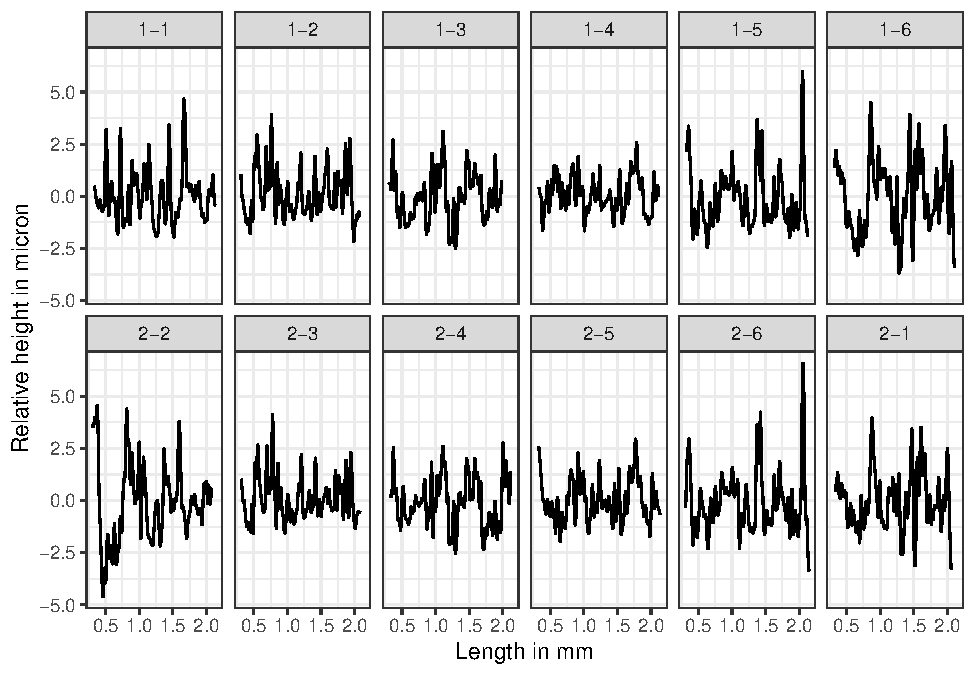
\includegraphics[width=\textwidth]{ju-hofmann_files/figure-latex/sigs-1} 

}

\caption[Signatures of all lands of bullet 1 in the top row, and of bullet 2 in the bottom row]{Signatures of all lands of bullet 1 in the top row, and of bullet 2 in the bottom row. Signatures in the second row are ordered to be in phase with the signatures above, i.e. matching signatures are displayed on top of each other.}\label{fig:sigs}
\end{figure}
\end{Schunk}

The signatures of Land 4 of Bullet 1 and Land 5 of Bullet 2 are stored
in objects \code{sigs2} and \code{sigs1}, respectively. This comparison
consists of a pair of signatures that are known to be a match -- a KM
(known match) comparison. We compute the CMPS score using two versions
of the CMPS algorithm:

\begin{Schunk}
\begin{Sinput}
sigs1 <- bullets$sigs[bullets$bulletland == "2-5"][[1]]
sigs2 <- bullets$sigs[bullets$bulletland == "1-4"][[1]]

# compute cmps

# algorithm with multi-peak insepction at three different segment levels
cmps_with_multi_scale <- 
  extract_feature_cmps(sigs1$sig, sigs2$sig, 
                       npeaks.set = c(5,3,1), include = "full_result")

# algorithm with multi-peak inspection at the basis scale only
cmps_without_multi_scale <- 
  extract_feature_cmps(sigs1$sig, sigs2$sig, 
                       npeaks.set = 5, include = "full_result")
\end{Sinput}
\end{Schunk}

In the first example, \code{npeaks.set} is a vector of three integers,
i.e.~the algorithm uses the multi-segment lengths strategy to create the
result object \code{cmps\_with\_multi\_scale}. For
\code{cmps\_without\_multi\_scale} each basis segment is linked to the
top 5 candidate positions. We use \code{include = "full\_result"} to
capture all results. In this example, the CMPS is 9 when using multiple
segments, and 12 when using a single segment. As discussed in
\citet{cmps}, using multi-segment lengths strategy can reduce the number
of false positives when identifying candidate positions; however, any
score based method is walking the line between false positives and false
negatives. As the number of false positives is reduced the number of
false negatives might rise. More discussion and comparisons between the
two versions of the CMPS algorithm will be presented in later sections.
Note, that the multi-segment lengths method is slower because the
algorithm is run once for each segment length.

\textbf{Visualize and understand CMPS results}

We also implemented graphing tools for visualizing results of the CMPS
algorithm. The goal is to provide users with tools to inspect each of
the basis segments and to help them have a better understanding of how
the algorithm works. \autoref{fig:sigplots} shows the plots generated by
the first graphing function, \code{cmps\_signature\_plot()}, and
continues with the example above. \code{cmps\_signature\_plot()} takes
the output of
\code{extract\_feature\_cmps(..., include = "full\_result")} and returns
a list of 5 elements. It creates an overall impression of how the
comparison signature aligns with the reference signature at the
congruent registration position.

\begin{itemize}
\item
  The first element is a plot called \code{segment\_shift\_plot}, shown
  in \autoref{fig:sigplot}. On this plot the reference signature is
  drawn as a black line, congruent matching profile segments from the
  comparison signature are overlaid in red at the congruent registration
  position.
\item
  The second plot is called \code{signature\_shift\_plot}, shown in
  \autoref{fig:sigplot2}. This visual presents both the comparison
  signature and the reference signature. The comparison signature is
  aligned with the reference signature based on the congruent
  registration position. Congruent matching profile segments are
  highlighted by solid red lines.
\end{itemize}

\begin{figure}[hbt]
\begin{subfigure}[t]{\textwidth}
\caption{\label{fig:sigplot}The black line shows the comparison signature; each red line segment shows one congruent matching profile segment.}
\vspace{1em}
\begin{adjustbox}{valign=t}
\begin{minipage}{.39\textwidth}

{\small {}
\begin{Schunk}
\begin{Sinput}
sig.plot <- cmps_signature_plot(
  cmps_with_multi_scale
)
sig.plot$segment_shift_plot
\end{Sinput}
\end{Schunk}
}
\vspace{1em}
\end{minipage}
\begin{minipage}{.59\textwidth}
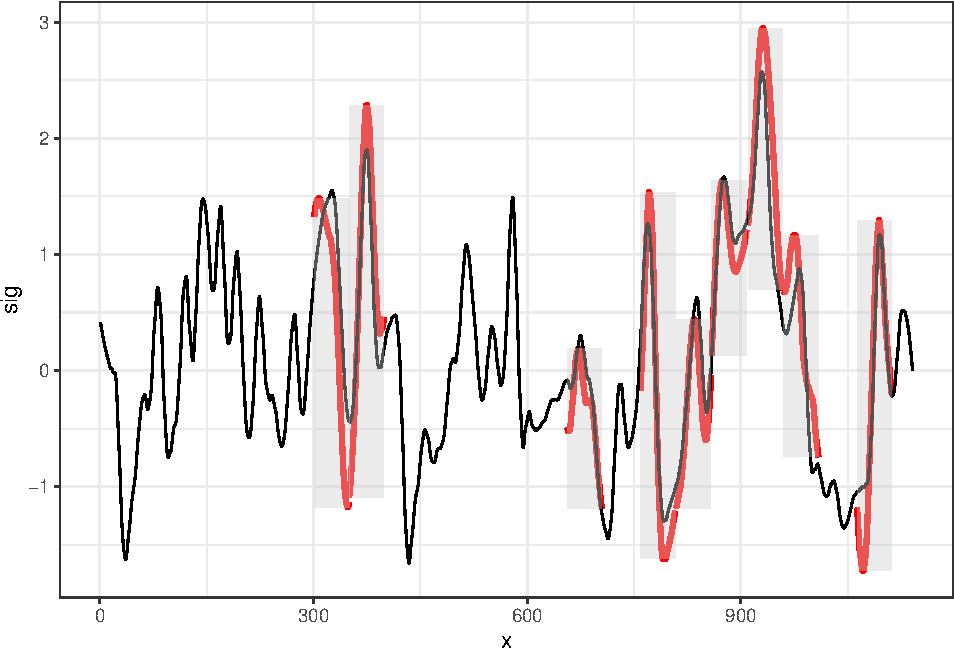
\includegraphics[width=\textwidth]{ju-hofmann_files/figure-latex/sigplot-1.pdf}
\end{minipage}
\end{adjustbox}
\end{subfigure}
\begin{subfigure}[t]{\textwidth}
\caption{\label{fig:sigplot2}The black line shows the reference signature; the red line shows the comparison signature. Solid part shows the congruent matching profile segments, and the dashed part shows segments that do not agree with the congruent registration position.}
\vspace{1em}
\begin{adjustbox}{valign=t}
\begin{minipage}{.39\textwidth}

{\small {}
\begin{Schunk}
\begin{Sinput}
sig.plot$signature_shift_plot
\end{Sinput}
\end{Schunk}
}
\vspace{1em}
\end{minipage}
\begin{minipage}{.59\textwidth}
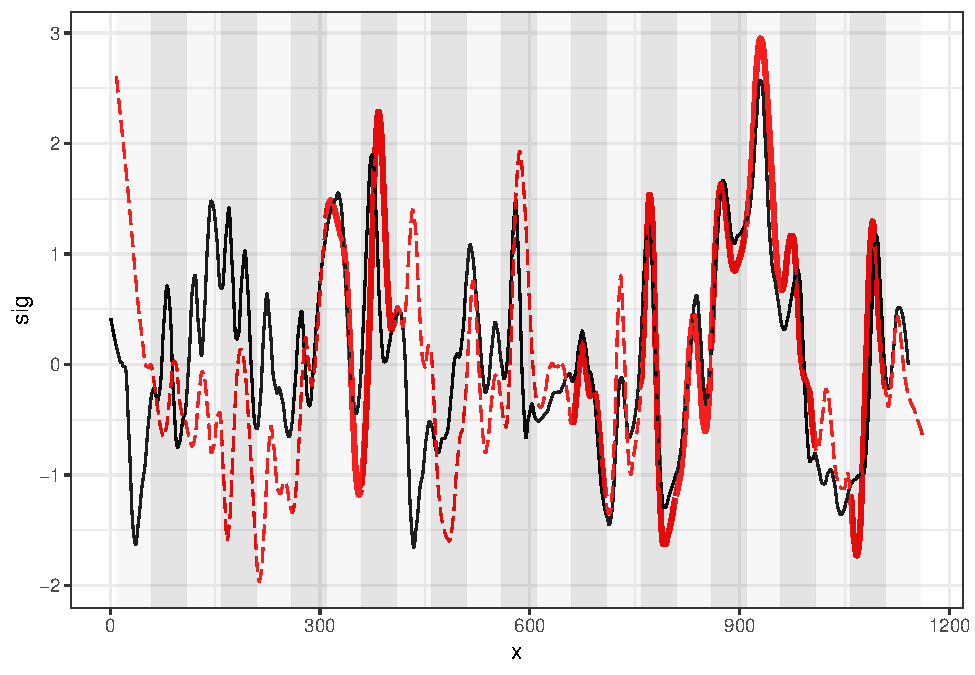
\includegraphics[width=\textwidth]{ju-hofmann_files/figure-latex/sigplot2-1.pdf}
\end{minipage}
\end{adjustbox}
\end{subfigure}
\caption{\label{fig:sigplots} Two visual outputs of cmps\_signature\_plot()}
\end{figure}

\begin{itemize}
\tightlist
\item
  Other elements of this list are \code{seg\_shift} and
  \code{sig\_shift}. \code{sig\_shift} gives the congruent registration
  position, while \code{seg\_shift} is a data frame showing the
  congruent matching profile segments and their identified candidate
  position closest to the congruent registration position.
\end{itemize}

\begin{Schunk}
\begin{Sinput}
sig.plot$seg_shift
\end{Sinput}
\begin{Soutput}
#>    seg.idx seg.shift
#> 7        7         0
#> 8        8        -1
#> 14      14         5
#> 16      16         8
#> 17      17         8
#> 18      18         8
#> 19      19         9
#> 20      20         9
#> 22      22        12
\end{Soutput}
\end{Schunk}

While \code{cmps\_signature\_plot()} focuses on the signature level,
\code{cmps\_segment\_plot()} focuses on the segment level. It provides
the ``full result'' of \code{extract\_feature\_cmps()}, but also takes
an argument, \code{seg.idx}, indicating which segment should be
inspected. When checking \code{sig.plot\$seg\_shift} we notice that
segment number 6 is not one of the congruent matching profile segments.
We can therefore set \code{seg.idx = 6} in \code{cmps\_segment\_plot()}
and investigate the reason why this segment disagrees with the congruent
registration position.

For each segment scale, we have two plots: \code{segment\_plot} and
\code{scale\_ccf\_plot}, as shown in \autoref{fig:segplots} for the
example of segment number 6:

\begin{itemize}
\tightlist
\item
  \autoref{fig:segplot} is the \code{segment\_plot} for basis segment 6
  at level one (in its original length). We used
  \code{npeaks.set = c(5, 3, 1)} in \code{extract\_feature\_cmps()} when
  calculating the CMPS score. Therefore the top five peaks are
  identified in the cross-correlation curve at level one. Segment 6 is
  plotted at the positions where these 5 peaks are identified with
  dashed lines in the \code{segment\_plot}. The solid thick black line
  shows the segment at its original position (which in this example is
  very close to the actual registration position).
\item
  \autoref{fig:segplot2} is the \code{scale\_ccf\_plot} of basis segment
  6 at level one. It shows the cross-correlation curve computed by the
  reference signature and the level-one basis segment 6. The five
  highest peaks are marked by dots on the curve.
\end{itemize}

\begin{figure}
\begin{subfigure}[t]{\textwidth}
\caption{\label{fig:segplot}segment\_plot for segment 6 at level one. The original position of segment 6 is indicated by the solid black line. Positions where the segment achieves the 5 highest cross-correlations are indicated by the dashed line segments.}
\vspace{1em}
\begin{adjustbox}{valign=t}
\begin{minipage}{.39\textwidth}

{\small {}
\begin{Schunk}
\begin{Sinput}
seg.plot <- cmps_segment_plot(
  cmps_with_multi_scale, 
  seg.idx = 6
)
seg.plot[[1]]$segment_plot
\end{Sinput}
\end{Schunk}
}
\vspace{1em}
\end{minipage}
\begin{minipage}{.59\textwidth}
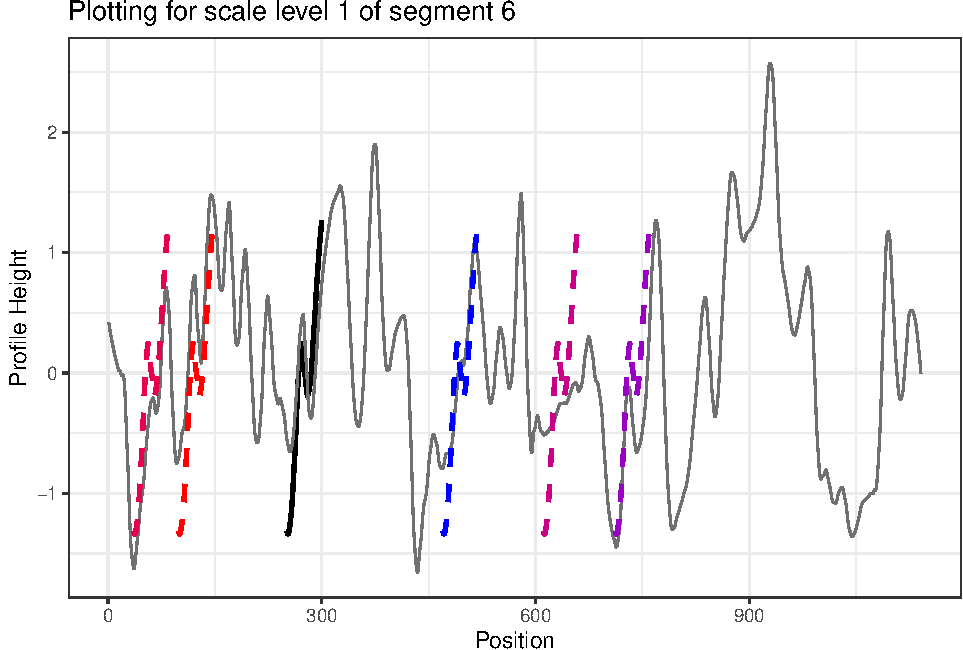
\includegraphics[width=\textwidth]{ju-hofmann_files/figure-latex/segplot-1.pdf}
\end{minipage}
\end{adjustbox}
\end{subfigure}
\begin{subfigure}[t]{\textwidth}
\caption{\label{fig:segplot2}scale\_ccf\_plot shows the cross-correlation curve between the reference signature and segment 6 at level one. The five highest peaks are marked by dots. The vertical red dashed line indicates the congruent registration position; the green dashed line shows a peak position in the highest segment level; the blue dashed lines show the tolerance zone around the green dashed line. We can see that none of the five highest peaks at level one falls within the tolerance zone, indicating that there is no consistent correlation peak or a candidate position identified by basis segment 6 under the multi-segment lengths strategy. Thus, the basis segment 6 doesn't vote for the congruent registration position and is not a cmps.}
\vspace{1em}
\begin{adjustbox}{valign=t}
\begin{minipage}{.39\textwidth}

{\small {}
\begin{Schunk}
\begin{Sinput}
seg.plot[[1]]$scale_ccf_plot
\end{Sinput}
\end{Schunk}
}
\vspace{1em}
\end{minipage}
\begin{minipage}{.59\textwidth}
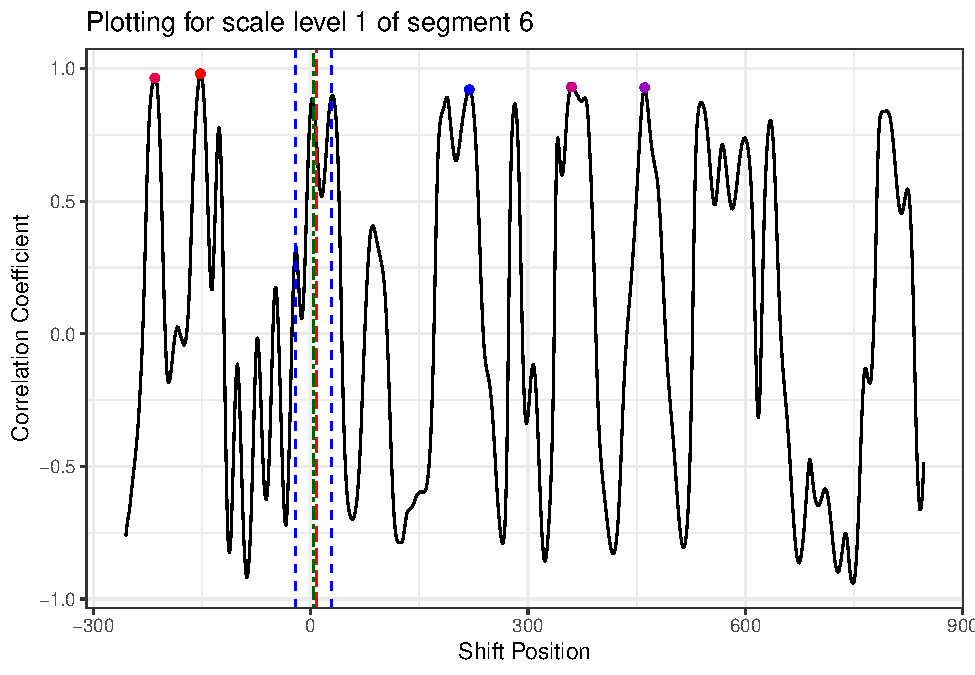
\includegraphics[width=\textwidth]{ju-hofmann_files/figure-latex/segplot2-1.pdf}
\end{minipage}
\end{adjustbox}
\end{subfigure}
\caption{\label{fig:segplots} Two plots used to investigate basis segment 6 at level one}
\end{figure}

Additionally, users can have more insights about why segment 6 is not a
congruent matching profile segment if we put the \code{segment\_plot}
and \code{scale\_ccf\_plot} of all three segment levels together, as
shown in \autoref{fig:seg_all} with the help of
\code{ggpubr::ggarrange()}.

\begin{figure}
\vspace{1em}
\begin{adjustbox}{valign=t}
\begin{minipage}{.39\textwidth}

{\small {}
\begin{Schunk}
\begin{Sinput}
library(ggpubr)

ggarrange(
  plotlist = 
    unlist(seg.plot, 
           recursive = FALSE),
  ncol = 2, 
  nrow = 3)
\end{Sinput}
\end{Schunk}
}
\vspace{1em}
\end{minipage}
\begin{minipage}{.59\textwidth}
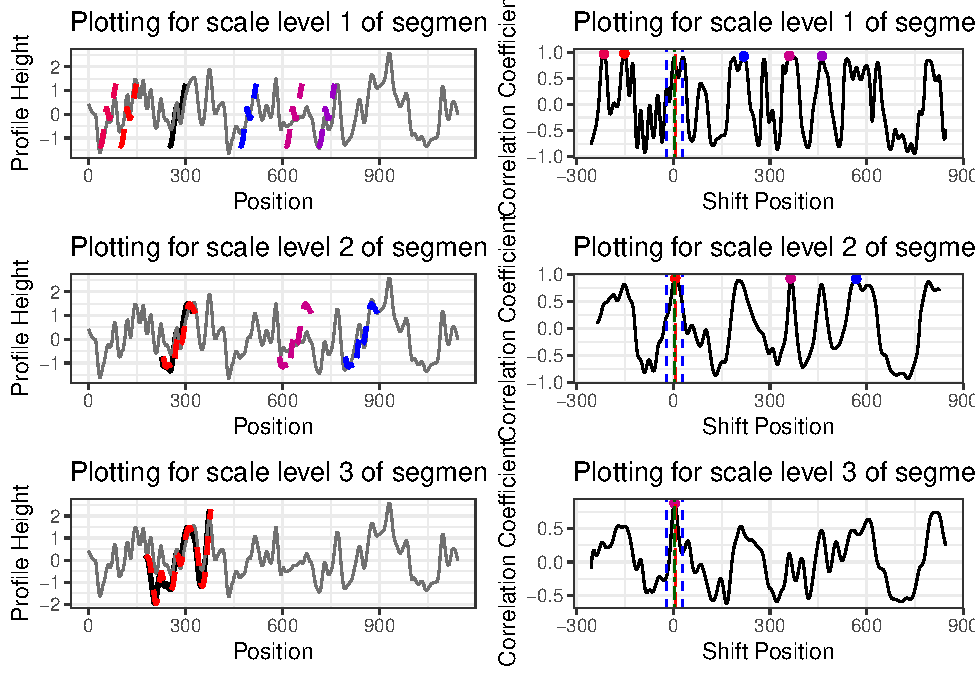
\includegraphics[width=\textwidth]{ju-hofmann_files/figure-latex/segplot3-1.pdf}
\end{minipage}
\end{adjustbox}
\caption{\label{fig:seg_all} Put segment\_plot and scale\_ccf\_plot of all three levels together. We are identifying five highest peaks at level one, three peaks at level two, and one peak at level three since npeaks.set = c(5, 3, 1). The highest peak position at level three is marked by the green dashed line across all segment levels. However, the highest peak on level three does not coincide with any of the top five highest peaks at level one. This indicates that there is no consistent correlation peak or a candidate position for basis segment 6 under the multi-segment lengths strategy.}
\end{figure}

In \autoref{fig:seg_all}, the red vertical dashed line indicates the
congruent registration position. We can see that the basis segment 6
does obtain a peak near the congruent registration position at level two
and level three, respectively; however, this position doesn't give one
of the five highest peaks at level one. As a result, segment 6 fails to
identify the consistent correlation peak (ccp) and fails to become one
of the congruent matching profile segments according to the
multi-segment lengths strategy. The identified top five peaks at level
one are also examples of ``false positive'' peaks. The ``true positive''
peak (the peak within the tolerance zone of the congruent registration
position) is identified at level two and three by increasing the segment
length, which justifies the usage of multi-segment lengths strategy.

\hypertarget{evaluation-metrics}{%
\subsection{Evaluation metrics}\label{evaluation-metrics}}

\textbf{Metrics based on CMPS scores}

The CMPS algorithm measures the similarity between two signatures
resulting in a similarity score of a land-to-level comparison. Bullets
fired from traditionally rifled barrels have multiple land and groove
engraved areas. Here, we are working with bullets fired from Ruger P85
barrels with six lands and grooves. A comparison of two bullets
therefore involves 36 land-to-land comparisons, resulting in 36 CMPS
scores (as shown in \autoref{fig:tiles}). In order to obtain a single
similarity score of a bullet-level comparison, we need to summarize
these 36 CMPS scores. Two similarity metrics for bullet-level
comparisons have been introduced in the literature \citep{cmps}:
\(\mathrm{CMPS_{max}}\) and \(\mathrm{\overline{CMPS}_{max}}\).
\(\mathrm{CMPS_{max}}\) is the highest CMPS score obtained among all
land-level comparisons, while \(\mathrm{\overline{CMPS}_{max}}\) is the
highest possible mean CMPS score of land-level comparisons that are in
the same phase:

In general, we assume each bullet has \(n\) land engravings (in our case
\(n=6\)). Let \(c_{ij}\) denote the CMPS score of a comparison between
bullet 1 land \(i\) and bullet 2 land \(j\), for \(i,j = 1, \dots, n\).
Let \(\mathcal{P}_k\) denote bullet land pairs in phase \(k\) for
\(k = 0, \dots, n-1\), and
\(\mathcal{P}_k = \{ (i,j): i = 1, \dots, n ; j = (i + k) - n \cdot \mathbbm{1}_{i + k > n} \}\),
where \(\mathbbm{1}_A\) denotes an indicator function. For example,
\(\mathcal{P}_1 = \{ (1,2), (2,3), (3,4), (4,5), (5,6), (6,1) \}\) when
\(n = 6\). Let \(k^*\) denote the index of the highest phase.

With that, the two measures to evaluate accuracy used in \citet{cmps}
are defined as

\begin{align}
\mathrm{CMPS_{max}} &= \max_{i,j} c_{ij} \text{ , and} \\
\mathrm{\overline{CMPS}_{max}} &= \frac{1}{n} \sum_{(i,j) \in \mathcal{P}_{k^*}} c_{ij} \text{ , where} \\
k^* &= \text{arg}\max\limits_{k} \left[  \frac{1}{n} \sum_{(i,j) \in \mathcal{P}_k} c_{ij}\right]
\end{align}

We can continue with the example used in previous sections.
\code{bullets} contains bullet signatures of two bullets, \code{bullet1}
and \code{bullet2}. As mentioned before, each bullet has 6 land
engravings, resulting in 6 bullet signatures. Thus, there are 36
pairwise bullet signature comparisons, resulting in 36 \(c_{ij}\) values
in total. We use multi-segment lengths strategy with default parameters
to compute these CMPS scores, and the result is shown in
\autoref{fig:tiles}. We can see that in this example,

\[
\mathrm{CMPS_{max}} =  \max_{i,j} c_{ij} = 17
\]

and since bullet lands in phase \(\mathcal{P}_1\) gives the highest mean
CMPS score (\(k^* = 1\)), we have

\[
\begin{aligned}
\mathrm{\overline{CMPS}_{max}} &= \frac{1}{6} \sum_{(i,j) \in \mathcal{P}_1} c_{ij} \\
                        &= \frac{1}{6} (c_{12} + c_{23} + c_{34} + c_{45} + c_{56} + c_{61}) \\
                        &= \frac{1}{6} (3+17+14+10+15+16) \\
                        &= 12.5
\end{aligned}
\]

\begin{Schunk}
\begin{figure}

{\centering 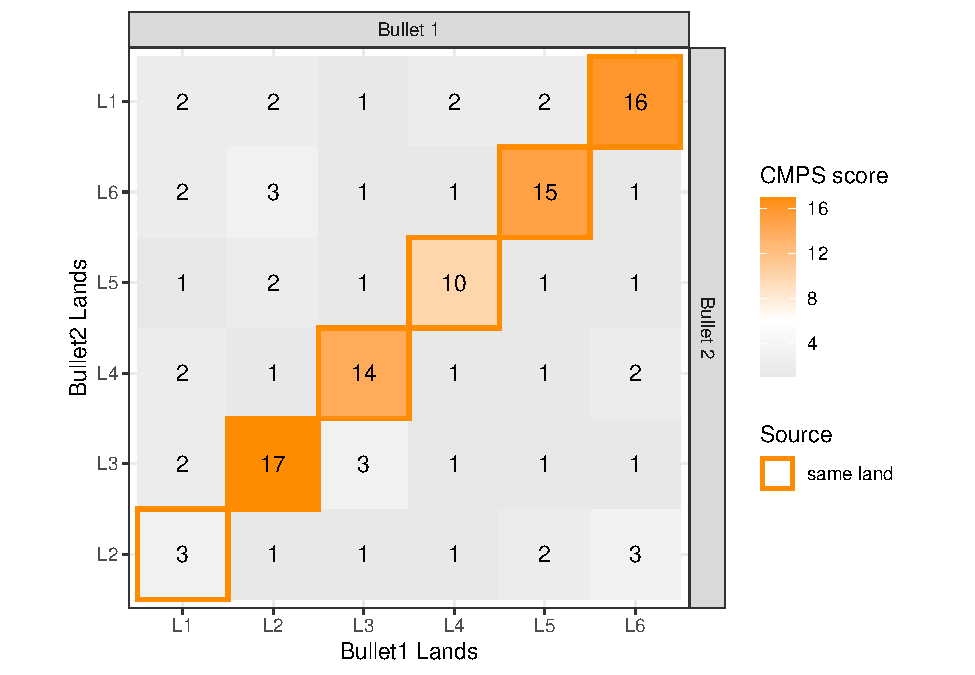
\includegraphics[width=.7\textwidth]{ju-hofmann_files/figure-latex/tiles-1} 

}

\caption[CMPS scores of all 36 pairwise bullet signature comparisons for two bullets]{CMPS scores of all 36 pairwise bullet signature comparisons for two bullets. Land engraving pairs generated by the same land (KM comparisons) are highlighted}\label{fig:tiles}
\end{figure}
\end{Schunk}

However, both \(\mathrm{CMPS_{max}}\) and
\(\mathrm{\overline{CMPS}_{max}}\) consider only relatively high CMPS
scores and ignore the rest. So we introduce a new metric based on CMPS
scores called \(\mathrm{\overline{CMPS}_{diff}}\), which is the
difference between \(\mathrm{\overline{CMPS}_{max}}\) and the mean of
all other CMPS scores. With our notation above, we have:

\begin{align}
\mathrm{\overline{CMPS}_{diff}} = \left[  \frac{1}{n} \sum_{(i,j) \in \mathcal{P}_{k^*}} c_{ij}\right] - \left[  \frac{1}{n(n-1)} \sum_{(i,j) \notin \mathcal{P}_{k^*}} c_{ij}\right]
\end{align}

\(\mathrm{\overline{CMPS}_{diff}}\) highlights the difference between
CMPS scores of matching and non-matching comparisons. If two bullets are
non-matching, all 36 CMPS scores are expected to be small with
relatively the same values, resulting in a
\(\mathrm{\overline{CMPS}_{diff}}\) value close to 0. For the example
above, \(\mathrm{\overline{CMPS}_{diff}} = 12.5 - 1.53 = 10.97\)

\textbf{Scaled CMPS scores}

Another issue with the CMPS score is that the highest possible CMPS
score (the total number of basis segments) might differ across
comparisons (as shown in \autoref{fig:tiles2}(a)) due to different
lengths of bullet signatures and different lengths of basis segments
specified by the parameter. A CMPS score of 5 might indicate a non-match
if the highest possible CMPS score is 30 but indicate a match if the
highest possible CMPS score is 6. Thus, we introduce the scaled CMPS
score, denoted as \(c^*_{ij}\). Let \(s_{ij}\) denote the highest
possible CMPS score or the total number of basis segments, then the
scaled CMPS score \(c^*_{ij}\) is defined as the ratio of raw score and
maximum score:

\begin{align}
c^*_{ij} = \frac{c_{ij}}{s_{ij}}
\end{align}

The scaled CMPS scores of the above example are shown in
\autoref{fig:tiles2}(b). Compared to the original CMPS scores, scaled
scores have values within the interval \([0, 1]\) regardless of the
length of the basis segments and therefore make a comparison of values
possible across different parameter choices. Similarly to the original
CMPS scores, we will denote the scaled CMPS scores adjusted for
out-of-phase background values by \(\mathrm{\overline{CMPS^*}_{diff}}\).
For example, \(\mathrm{\overline{CMPS^*}_{diff}} = 0.498\) for
\autoref{fig:tiles2}(b)

\begin{Schunk}
\begin{figure}

{\centering 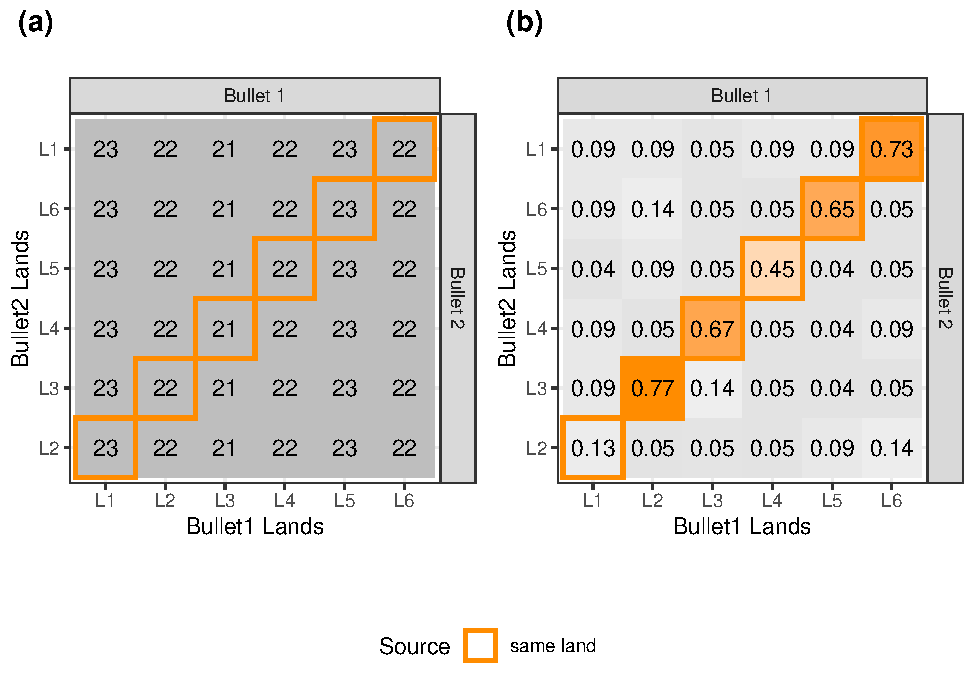
\includegraphics[width=.7\textwidth]{ju-hofmann_files/figure-latex/tiles2-1} 

}

\caption[Plot (a) shows the highest possible CMPS scores (the total number of basis segments) for the 36 comparisons]{Plot (a) shows the highest possible CMPS scores (the total number of basis segments) for the 36 comparisons. (b) shows the scaled CMPS scores for the 36 comparisons.}\label{fig:tiles2}
\end{figure}
\end{Schunk}

\textbf{Sum of squares ratio}

The ``sum of squares ratio'' quantifies how well two groups of values
separate. Let \(n_T\) denote the total number of observations, \(n_k\)
denote the number of observations in group \(k\), and \(y_{kl}\) denote
the \(l\)-th observation in group \(k\), for \(k = 1,2\) and
\(l = 1, \dots, n_k\). Let
\(\bar{y}_{k.} = \frac{1}{n_k} \sum_{l=1}^{n_k} y_{kl}\) denote the mean
value in group \(k\) and
\(\bar{y}_{..} = \frac{1}{n_T} \left( \sum_{k} \sum_{l = 1}^{n_k} y_{kl} \right)\)
denote the mean value of all observations. Consider the following model:

\begin{align}
y_{kl} = \mu_k + e_{kl}
\end{align}

where \(\mu_k\) is the true mean of group \(k\) and \(e_{kl}\) is a
random effect of different observations. Then we can define the sum of
squares ratio \(V\) as:

\begin{align}
V = \frac{\sum_k n_k (\bar{y}_{k.} - \bar{y}_{..})^2}{\sum_k \sum_l^{n_k} (y_{kl} - \bar{y}_{k.})^2 }.
\end{align}

The numerator of the sum of squares ratio \(V\) quantifies the variation
between the two groups, while the denominator quantifies the variation
within each group. The sum of squares ratio \(V\) can be used as an
index for evaluating scans, metrics, and different sets of parameters if
the same data set is being used. Some examples will be presented in the
following section. If we impose the normality and independence
assumptions on the random effects \(e_{kl}\), the sum of squares ratio
\(V\) becomes a scaled F-statistic with degrees of freedom of \(k-1\)
and \(n_T - k\) and \(F = \frac{n_T - k}{k- 1} V\). If we want to
compare different data sets, stating that a certain setup can achieve
better separation on one data set than another, we can scale the sum of
squares ratio \(V\) and obtain the F-statistic to compare the p-values.

Using the sum of squares ratio \(V\) as an evaluation metric, we are
able to construct a pipeline that aims to find the optimal parameter
value for the CMPS algorithm by maximizing the sum of squares ratio. In
the following section, we will use this ratio to compare the CMPS
metrics introduced earlier and investigate effects of different sets of
parameters.

\hypertarget{results}{%
\subsection{Results}\label{results}}

As presented in the work of \citet{cmps}, researchers applied the CMPS
method to scans of one of the Hamby sets. While it is not explicitly
stated in the paper, we presume this to be Hamby 252, as only those
scans were publicly available at the time. In order to show that our
implementation of the CMPS algorithm is able to reproduce the results in
\citet{cmps} and be used for other data sets, we applied our
implementation to both Hamby set 252 and Hamby set 44. For the purpose
of reproducibility, we present how we obtained bullet signatures from
the Hamby set data and include code in the appendix: for both Hamby 252
and Hamby 44, we started with scans in the form of x3p files in the
database. Following the framework proposed by \citet{aoas}, we used the
same set of parameters, removed damaged bullet scans, obtained bullet
signatures for each bullet land engraving, and removed outliers in
bullet signatures. Note that researchers of \citet{cmps} applied the
CMPS algorithm to bullet signatures as well but used a framework
different from ours. However, since their work is not open-source, we
were not able to follow their framework and were only able to reproduce
the results for Hamby set 252 qualitatively.

\textbf{Hamby 252}

\autoref{fig:result1_252} shows the distribution of
\(\mathrm{CMPS_{max}}\) and \(\mathrm{\overline{CMPS}_{max}}\) after we
applied the CMPS algorithm to Hamby set 252 with the multi-segment
lengths strategy. The parameters we used in
\code{extract\_feature\_cmps} for the CMPS algorithm are:

\begin{Schunk}
\begin{Sinput}
extract_feature_cmps(
  x, y,
  seg_length = 50,
  Tx = 25,
  npeaks.set = c(5,3,1),
  include = "nseg"
)
\end{Sinput}
\end{Schunk}

As noted above, the CMPS scores we found here are not exactly the same
as those presented in \citet{cmps} since we were not able to follow
their framework, but the results presented in \autoref{fig:result1_252}
are qualitatively equivalent to those presented in \citet{cmps}, showing
a clear separation between scores based on comparisons from known
matches (KM) and scores from comparisons of known non-matches (KNM) for
both \(\mathrm{CMPS_{max}}\) and \(\mathrm{\overline{CMPS}_{max}}\).

Additionally, to mimic the parameters used in \citet{cmps}, we set
\code{seg\_length = 50} and \code{Tx = 25} to make sure that each basis
segment has length of 78.125 \textmu m and the tolerance zone is
\(\pm 39.0625\) \textmu m (one unit represents 1.5625 \textmu m for
Hamby set 252).

The sum of squares ratios are 20.64 and 28.96 for
\(\mathrm{CMPS_{max}}\) and \(\mathrm{\overline{CMPS}_{max}}\),
respectively. This indicates, that even though scores from
\(\mathrm{CMPS_{max}}\) for known-match comparisons are larger than
scores from the averaged version of \(\mathrm{\overline{CMPS}_{max}}\),
these scores achieve a better separation between the two groups of
comparisons.

\begin{Schunk}
\begin{figure}

{\centering 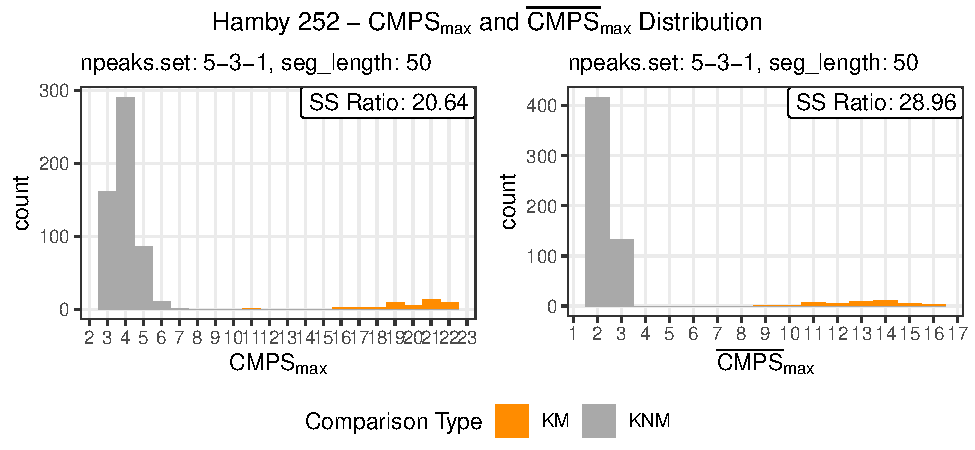
\includegraphics[width=400px]{ju-hofmann_files/figure-latex/result1_252-1} 

}

\caption{Distribution of $\mathrm{CMPS_{max}}$ and $\mathrm{\overline{CMPS}_{max}}$ for Hamby 252; outliers are removed in bullet signatures; \texttt{seg\_length = 50}, \texttt{Tx = 25}, \texttt{npeaks.set = c(5,3,1)} }\label{fig:result1_252}
\end{figure}
\end{Schunk}

\textbf{Hamby 44}

Similar procedures are applied to Hamby set 44, and
\autoref{fig:result1_44} shows the distribution of
\(\mathrm{CMPS_{max}}\) and \(\mathrm{\overline{CMPS}_{max}}\),
respectively. The parameters used in \code{extract\_feature\_cmps} are:

\begin{Schunk}
\begin{Sinput}
extract_feature_cmps(
  x, y,
  seg_length = 61, 
  Tx = 30,
  npeaks.set = c(5,3,1),
  include = "nseg"
)
\end{Sinput}
\end{Schunk}

Since the resolution of Hamby 44 is set to 1.29 \textmu m per unit, we
make \code{seg\_length = 61} and \code{Tx = 30} to ensure that the setup
of Hamby set 44 is similar to that of Hamby set 252, resulting in basis
segments of 78.69 \textmu m and the tolerance zone of \(\pm 38.7\)
\textmu m.

As shown in \autoref{fig:result1_44}, again, we are able to see a clear
separation between the known match comparisons and the known non-match
comparisons, even though the separation is relatively small compared
with that of Hamby set 252, which is also indicated by the sum of
squares ratios. For this specific set of parameters, the sum of squares
ratios are 8.87 and 10.64 for \(\mathrm{CMPS_{max}}\) and
\(\mathrm{\overline{CMPS}_{max}}\), respectively. This might suggest
that we could enlarge the separation in terms of the sum of squares
ratio by using other CMPS metrics and other sets of parameters.

\begin{Schunk}
\begin{figure}

{\centering 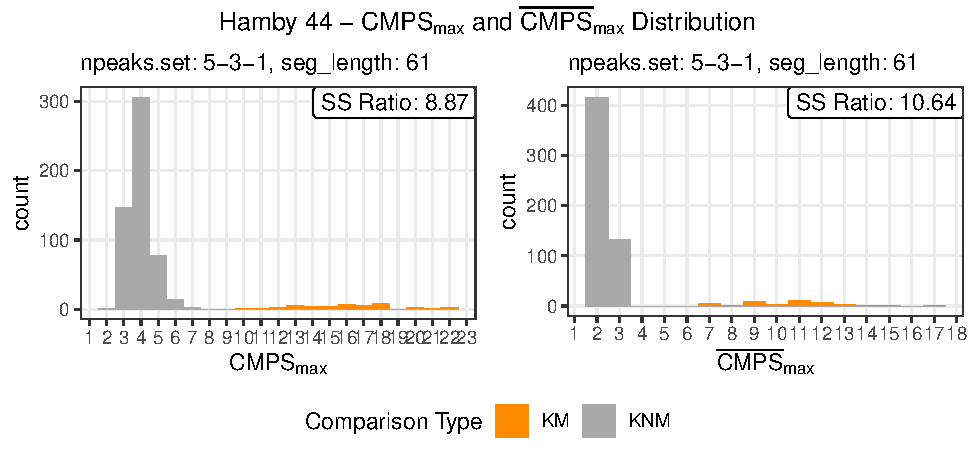
\includegraphics[width=400px]{ju-hofmann_files/figure-latex/result1_44-1} 

}

\caption{Distribution of $\mathrm{CMPS_{max}}$ and $\mathrm{\overline{CMPS}_{max}}$ for Hamby 44; outliers are removed in bullet signatures; \texttt{seg\_length = 61}, \texttt{Tx = 30}, \texttt{npeaks.set = c(5,3,1)} }\label{fig:result1_44}
\end{figure}
\end{Schunk}

\textbf{Comparing CMPS metrics and parameters}

\begin{Schunk}
\begin{figure}

{\centering 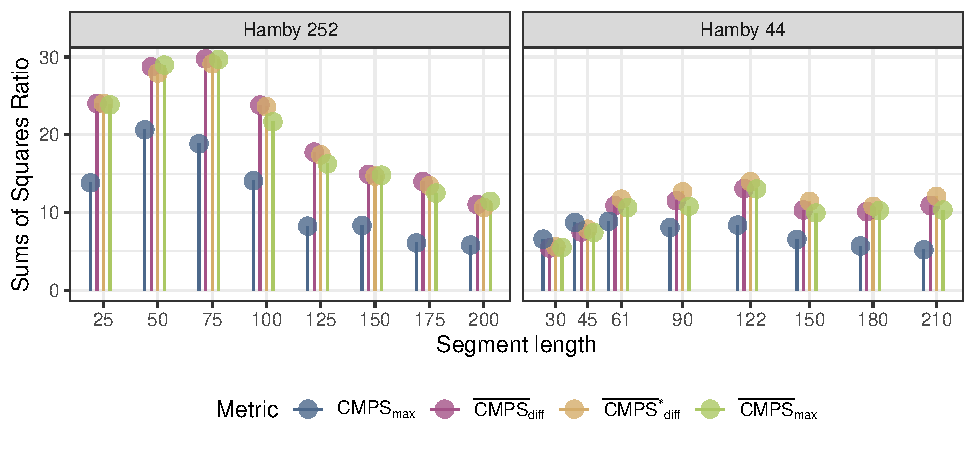
\includegraphics[width=400px]{ju-hofmann_files/figure-latex/param_seg_plot-1} 

}

\caption{Comparison of results from the CMPS algorithm based on different basis segment lengths (parameter \texttt{seg\_length}). Only the $\mathrm{CMPS_{max}}$ metric suggests that the default values for the basis segment length result in the best separation. Better separation is achieved based on the modified CMPS metrics, inclusing the newly suggested ones. For Hamby 252 these metrics agree on a segment length of 75, and a segment length of 122 for Hamby 44 yields better results}\label{fig:param_seg_plot}
\end{figure}
\end{Schunk}

\begin{Schunk}
\begin{figure}

{\centering 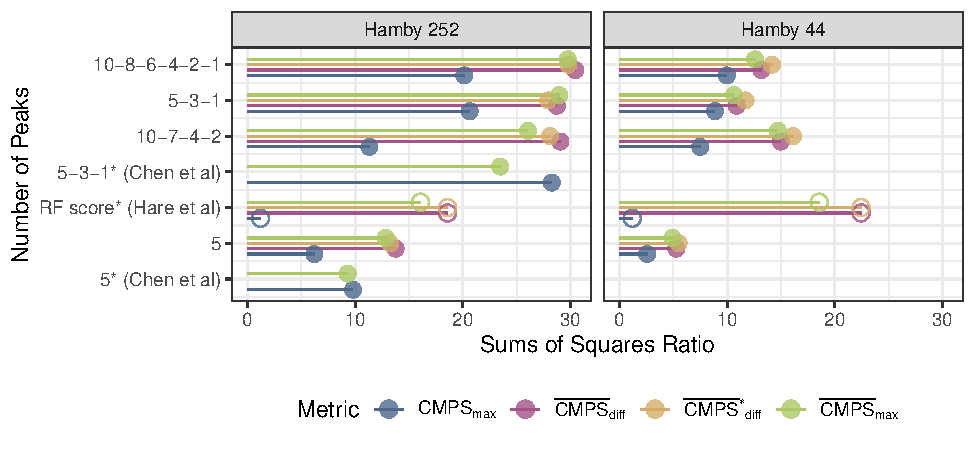
\includegraphics[width=400px]{ju-hofmann_files/figure-latex/param_npeak_plot-1} 

}

\caption[Comparison of CMPS results based on different strategies of number of peak selections]{Comparison of CMPS results based on different strategies of number of peak selections. Starred results compare CMPS performance with results published in the literature. Results for the random forest score are represented with circles because the metrics are computed not based on the CMPS scores, but the random forest scores with the same logic. Since random forest scores lie within the interval $[0, 1]$, scaling the random forest scores will not change the results.}\label{fig:param_npeak_plot}
\end{figure}
\end{Schunk}

We investigated the effects of different sets of parameters at the
example of both Hamby sets 252 and 44. More specifically, we
investigated the separation achieved using the \pkg{cmpsR}
implementation under various segment lengths (controlled by the
parameter \code{seg\_length}). Specifically, we fixed the parameter
\code{npeaks.set} that controls the number of peaks at each segment
level to be \code{npeaks.set = c(5,3,1)} and modified the parameter
\code{seg\_length}. \autoref{fig:param_seg_plot} shows that the default
values of \code{seg\_length} for Hamby 252 and Hamby 44 (50 for Hamby
252 and 61 for Hamby 44, which represent 78.125 \textmu m and 78.69
\textmu m, respectively) result in high values of the sum of squares
ratio, no matter which CMPS metrics are used for an evaluation. However,
we also see, that for Hamby set 252 a basis segment length of 75 is a
better choice than the default segment length; a basis segment length of
122 results in a higher value of sum of squares ratio for Hamby 44.

\autoref{fig:param_npeak_plot} shows results of the CMPS algorithm using
different strategies for identifying peaks in the correlation structure
between signatures. Basis segment length is fixed to the default level
for this evaluation. As can be seen in \autoref{fig:param_npeak_plot},
the default value of \code{npeaks.set} (\code{npeaks.set = c(5,3,1)})
leads to promising results in terms of the sum of squares ratio;
however, other choices of \code{npeaks.set} match and exceed this sum of
squares ratio value.

As seen before, the results suggest that the \(\mathrm{CMPS_{max}}\)
metric produces the least amount of separation compared with the other
three CMPS metrics. They also suggest that the two newly proposed
metrics, \(\mathrm{\overline{CMPS}_{diff}}\) and
\(\mathrm{\overline{CMPS^*}_{diff}}\), lead to equally good or even
better results as \(\mathrm{\overline{CMPS}_{max}}\). Because
\(\mathrm{\overline{CMPS^*}_{diff}}\) relies on a scaled version of CMPS
scores it is more comparable to other similarity scores and summarizes
the out-of-phase background CMPS scores, making it superior to the other
CMPS metrics.

What we can also observe in \autoref{fig:param_seg_plot} and
\autoref{fig:param_npeak_plot} is that the values of the sum of squares
ratio for Hamby 44 is lower than those for Hamby 252. This might be
because determining the source is a harder task for Hamby 44 than for
Hamby 252, but also suggests that the choice of parameters also depends
on the resolution or the scanning process of the data set. The same set
of parameters might work for one data set, but not work equally well for
another.

The purpose of the results shown in \autoref{fig:param_seg_plot} and
\autoref{fig:param_npeak_plot} is not to determine the ``best''
parameters for the CMPS algorithm, but to show that the sum of squares
ratio can be used as an evaluation measure to compare different
parameters, metrics, or scans. A pipeline that maximizes the sum of
squares ratio might help researchers determine the set of parameters
that work best for their data. But a large database that is
representative is what we really need in order to fully understand and
cross-validate the parameters of the CMPS algorithm.

\textbf{Comparing with original results and the random forest model}

\citet{cmps} present histograms of \(\mathrm{CMPS_{max}}\) and
\(\mathrm{\overline{CMPS}_{max}}\) for \code{npeaks.set = 5} and
\code{npeaks.set = c(5,3,1)} with (presumably) Hamby 252. The values in
these histograms allow us to calculate the sum of squares ratios and
include the results in \autoref{fig:param_npeak_plot} as well. They are
marked by an asterisk at the top right corner in
\autoref{fig:param_npeak_plot}. The sum of squares ratios we obtained
for \code{npeaks.set = 5} and \code{npeaks.set = c(5,3,1)} is slightly
higher than those obtained from the histograms of \citet{cmps}. It's
curious to see that for the Hamby 252 results published in \citet{cmps}
the \(\mathrm{{CMPS}_{max}}\) metric achieves values of the sum of
squares ratio higher than those achieved by the
\(\mathrm{\overline{CMPS}_{max}}\) metric.

Since the researchers of \citet{cmps} did not use
\(\mathrm{\overline{CMPS}_{diff}}\) or
\(\mathrm{\overline{CMPS^*}_{diff}}\), and they did not apply the CMPS
algorithm to the Hamby set 44, we were not able to compare those
results.

In \autoref{fig:param_npeak_plot}, we also included the sum of squares
ratios computed from the random forest scores \citep{aoas} for different
metrics. The random forest model presented in \citet{aoas} was trained
at the Center for Statistics and Applications in Forensic Evidence
(CSAFE) and is publicly available in the R package \pkg{bulletxtrctr}
\citep{bulletxtrctr}. Similarly to the CMPS algorithm, this random
forest model produces a score to quantify the similarity of a
land-by-land comparison. The RF scores lie in an interval of {[}0,1{]}
making them most comparable to the scaled CMPS scores. We applied the
logic of \(\mathrm{{CMPS}_{max}}\), \(\mathrm{\overline{CMPS}_{max}}\),
and \(\mathrm{\overline{CMPS}_{diff}}\) to the random forest scores and
obtained results of the random forest model for different metrics. As
shown in \autoref{fig:param_npeak_plot}, the random forest model does
not achieve the sum of squares ratio as high as those achieved by the
top CMPS algorithms for Hamby 252, but it does achieve better results
for Hamby 44. This might suggest that an inclusion of the CMPS score as
an additional feature in the random forest model training might be
beneficial for an overall separation to determine source.

The code generating all results of this manuscript can be found on
Github at
\url{https://github.com/willju-wangqian/CMPSpaper/tree/main/reproducible}

\hypertarget{conclusion}{%
\subsection{Conclusion}\label{conclusion}}

\hh{XXX Will, the conclusion needs to be a bit more than just a summary of what we did in the paper - think of it as a summary plus either the limitations of our approach, or next steps that should be done but goes beyond this paper.}

In this paper we present the \pkg{cmpsR} package, an open-source
implementation of the Congruent Matching Profile Segments (CMPS)
algorithm \citep{cmps}, and apply it to two datasets in Hamby study
\citep{hamby} to show its potential for further research. The CMPS
algorithm was proposed by NIST in 2019 and was made for objective tool
marks comparisons. We introduce the basic logic of the CMPS algorithm
and lay out its implementation in the \pkg{cmpsR} package. We also
showcase the functionality of the \pkg{cmpsR} package with a small
dataset example that is included in the package. In the \pkg{cmpsR}
package we implement some graphing tools for users to visualize results
and to gain a better understanding of both the algorithm and the
results.

\wj{Additionally, we propose new metrics based on the CMPS scores and compare the new metrics with the existing metrics. 
We also introduce a principled evaluation framework of algorithmic results using  a measure based on the sum of squares ratio. 
We showcase the implementation with two datasets in Hamby study (Hamby set 252 and Hamby set 44) and compare the CMPS algorithm using different sets of parameters and different metrics, following the evaluation framework based on the sum of squares ratio. }

The results obtained are promising: we were both able to reproduce the
results in \citet{cmps} qualitatively and achieve a clear separation
between the known match (KM) comparisons and known non-match (KNM)
comparisons in another bullet study.
\wj{However, the comparisons among different sets of parameters suggest that the optimal choice for parameter settings vary between different datasets. We propose an evaluation framework that allows a comprehensive cross-validation of parameter settings used in the algorithm for future research. 
Comparisons of the R implementation of the CMPS algorithm with the random forest model proposed by @aoas  suggest that adding the CMPS score as an additional feature in the random forest model might add further separation between known match (KM) comparisons and known non-match (KNM) comparisons.}

\wj{The open-source implementation of the CMPS algorithm provided by the \pkg{cmpsR} package is just one step towards in the framework of open science. Open science is particularly important to fields like forensic science where transparency and accuracy are critical to fair justice. 
Open-source implementations not only allow a peer-review but also facilitate further research, such as parameter cross-validations, method comparisons, and the development of statistical methods for modeling KM and KNM CMPS score distributions, which can then be used for error-rate estimations and fair applications that were called for by the PCAST [@pcast] report.
However, having open-source implementations is not enough for open science. 
In order to actually build the world of open science, many other efforts, such as open evaluation, open access publication, open educational resources, etc., are still needed. 
The database built and maintained by the National Institute of Standards and Technology is a good example of open data. 
What we are aiming for is an open system that is able to collect open results, compare multiple algorithms using multiple datasets, and evaluate algorithmic variation and accuracy. 
The evaluation metric we proposed in this paper can be used to compare different algorithms or even different datasets and is a snippet of this open system. 
But the core of this open system is the open science culture and contributions of the community.}

\bibliography{ju-hofmann.bib}

\address{%
Wangqian W. Ju\\
Department of Statistics\\%
Center for Statistics and Applications in Forensic Evidence\\ Iowa State
University\\ 2438 Osborn Dr\\ Ames, IA 50011\\
%
\url{https://github.com/willju-wangqian}%
\\\textit{ORCiD: \href{https://orcid.org/0000-0002-9977-377X}{0000-0002-9977-377X}}%
\\\href{mailto:wju@iastate.edu}{\nolinkurl{wju@iastate.edu}}
}

\address{%
Heike Hofmann\\
Department of Statistics\\%
Center for Statistics and Applications in Forensic Evidence\\ Iowa State
University\\ 2438 Osborn Dr\\ Ames, IA 50011\\
%
\url{https://github.com/heike}%
\\\textit{ORCiD: \href{https://orcid.org/0000-0002-9079-593X}{0000-0002-9079-593X}}%
\\\href{mailto:hofmann@iastate.edu}{\nolinkurl{hofmann@iastate.edu}}
}
